\documentclass{standalone}
\usepackage{tikz} % Import the tikz package
\usetikzlibrary{automata} % Import library for drawing automata
\usetikzlibrary{positioning} % ...positioning nodes
\usetikzlibrary{arrows} % ...customizing arrows
\tikzset{node distance=2.5cm,
    every state/.style={
        semithick,
        fill=gray!10},
    initial text={},
    double distance=2pt,
    every edge/.style={
        draw,
        ->,>=stealth',
        auto,
        semithick}}
\let\epsilon\varepsilon
\begin{document}
    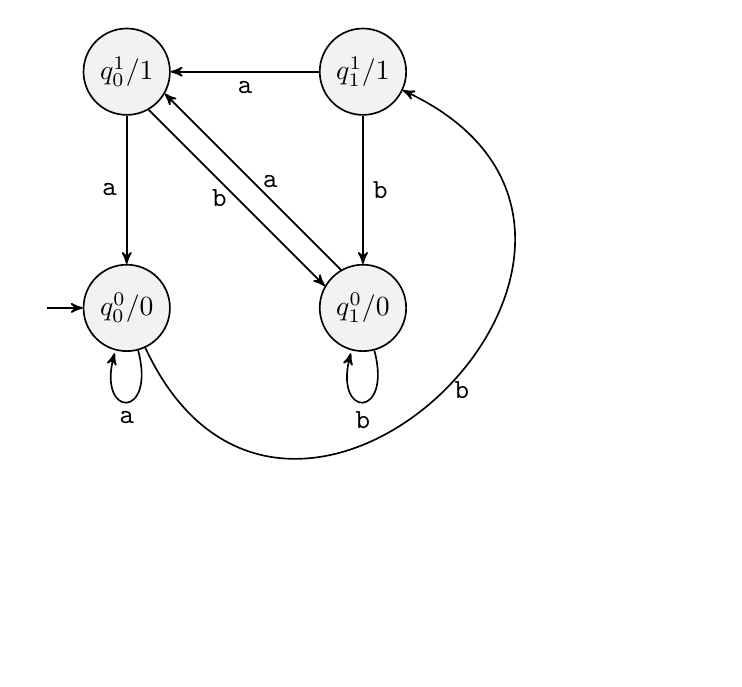
\begin{tikzpicture}
        \node[state,initial] (q00) at (0,0) {$q_0^0/0$};
        \node[state] (q01) at (0,3) {$q_0^1/1$};
        \node[state] (q10) at (3,0) {$q_1^0/0$};
        \node[state] (q11) at (3,3) {$q_1^1/1$};
        
        \draw (q01) edge[left] node {\tt a} (q00);
        \draw (q01.300) edge[left] node {\tt b} (q10.150);

        \draw (q00) edge[loop below] node {\tt a} (q00);
        \draw (q00) edge[bend left=250,looseness=2.4,right] node {\tt b} (q11);

        \draw (q10) edge[loop below] node {\tt b} (q10);
        \draw (q10.120) edge[right] node {\tt a} (q01.330);

        \draw (q11) edge[] node {\tt a} (q01);
        \draw (q11) edge[] node {\tt b} (q10);
    \end{tikzpicture}
\end{document}